\documentclass[a4paper,11pt,oneside]{book}

%% Zeichenkodierung

\usepackage[latin1]{inputenc}

%% Deutsches Sprachpaket
\usepackage[german]{babel}

%% Grafik-Einbindung
\usepackage{graphicx}

%% Mathe-Einbindung
\usepackage{amsmath,amsfonts,amssymb,bbm}

%% Schriftart �ndern auf Computer Modern Sans Serif
\usepackage[T1]{fontenc}
\renewcommand*\familydefault{\sfdefault}

%% Metadaten des Dokuments
\title{Kurztitel}
\author{Max Mustermann}
\date{SoSe 2012}

%% Literaturverzeichnis nach nature-Vorbild
\usepackage[square,numbers,sort&compress]{natbib}
\bibliographystyle{abbrvnat}

%% Einzug nach Absatz und Zwischenraum
\setlength{\parindent}{0pt}
\setlength{\parskip}{8pt}

%% mytitle Kommando um den Autor zu �bernehmen
\newcommand{\writer}[1]{%
\vspace*{-10mm}\hspace*{10mm}\hfill{\normalfont bearbeitet von \emph{#1}}%
}

\begin{document}

%% Kopfzeile und Seitenzahlen
\pagestyle{headings}
\renewcommand{\chaptermark}[1]{\markright{#1}{}}
\pagenumbering{arabic}

%% Sample
\chapter{Range Minimum Query}
\writer{Felix Lauenroth \& Michael Mardaus}

\section{Einleitung}

Im Folgenden besch�ftigen wir uns mit dem \emph{Range Minimum Query} Algorithmus und dem Skyline Problem. In Kapitel 1 definieren wir zun�chst die Range Minimum Query und zeigen verschieden performante Implementierungsans�tze. Kapitel 2 behandelt das Skyline Problem und zeigt unsere Umsetzung.

\section{Definition}

 Kommen wir zun�chst zur Definition der \textbf{Range Minimum Query} (kurz: RMQ). Gegeben sei ein Array, innerhalb welchem die Indexposition des kleinsten Wertes eines gegebenen Intervalls $[\ell, r]$ gesucht wird --- oder mathematisch ausgedr�ckt:

\[\text{RMQ}_{A}(\ell,r) = \text{arg} \ \min_{\ell \leq k \leq r } A[k] \]

\vspace{-3mm}


\begin{figure}[h]
\begin{center}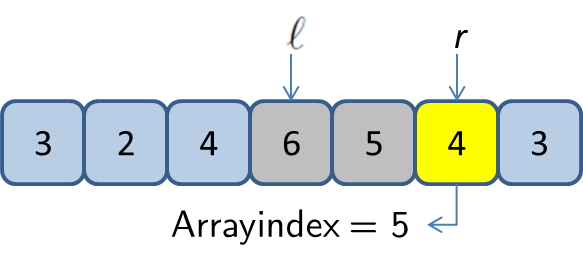
\includegraphics[width=5cm]{picture/array5.png}
\caption{Beispiel $\text{RMQ}_A(3,5) = 5$}
\label{definition}
\end{center}
\end{figure}


\section{Naive Ans�tze}
\subsection{Linear durch das Array iterieren}

Die erste triviale Idee das Problem zu l�sen w�re vermutlich das sequenzielle Durchiterieren durch das gegebene Intervall mit Abspeichern der Indexposition des bis zum aktuellen Schritt gefundenen Minimums. Dies schaffen wir offensichtlich in Linearzeit, also $\Oh(n)$ \footnote{\label{foot:1} $n$ beschreibt hier die L�nge des Intervalls}.

Wie auf den ersten Blick erkennbar ist, variiert die Laufzeit mit der L�nge des gegebenen Intervalls. Bei mehrfacher Ausf�hrung der Abfrage auf dem gleichen Array verschlechtert sich die Laufzeit sogar um den erheblichen Faktor $m$, wobei $m$ die Anzahl der Abfragen sei. Dies f�hrt somit zu einer Laufzeit von $\Oh(n\cdot m)$ bei $m$ Abfragen. Doch diese Methode hat auch einen Vorteil gegen�ber der folgenden Ans�tze. Sie funktioniert in-place, das hei�t sie ben�tigt nur eine konstante Menge an Speicher  (n�mlich dem des Arrays selbst), denn das Durchiterieren findet im Eingabearray selbst statt. Es wird nur ein zus�tzlicher Wert abgespeichert und zwar die Indexposition des bisher gefundenen Minimums.

\subsection{Preprocessing}

F�r wiederholte Abfragen auf das gleiche Eingabearray suchen wir nun Mechanismen, wie wir durch Vorausberechnen (dem sogenannten Preprocessing) zuk�nftige Abfragen mit verschiedenen Intervallgrenzen auf das gleiche Eingabearray beschleunigen k�nnen.

Wir ben�tigen hierf�r offensichtlich zus�tzlichen Speicher, in dem wir -- zum Beispiel in Form einer $n\times n$-Matrix -- alle Kominationen von Intervallgrenzen $\ell$ und $r$ und deren RMQ-Ergebnis abspeichern.

\begin{figure}[h]
\begin{minipage}{.5\textwidth}
\begin{center}
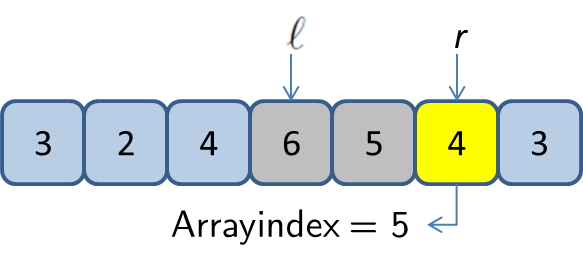
\includegraphics[width=5cm]{picture/array5.png}
\end{center}
\end{minipage}
\begin{minipage}{.5\textwidth}
\begin{center}
 $$
 \bordermatrix{
  &  &  &  &  &  & r &  \cr
  & 0 & 1 & 1 & 1 & 1 & 1 & 1 \cr
  &  & 1 & 1 & 1 & 1 & 1 & 1 \cr
  &  &  & 2 & 2 & 2 & 2 & 6 \cr
 \ell &  &  &  & 3 & 4 & \fbox{5} & 6 \cr
  &  &  &  &  & 4 & 5 & 6 \cr
  &  &  &  &  &  & 5 & 6 \cr
  &  &  &  &  &  &  & 6 }
 $$
\end{center}
\end{minipage}

\caption{Komplette $n\times n$-Matrix nach Preprocessing}
\label{prepro}
\end{figure}

Ab jetzt haben wir es also mit zwei verschiedenen Laufzeiten zu tun. Zum Einen der Laufzeit f�r eine Suchanfrage zum Auffinden der L�sung in der zuvor erstellten L�sungsmatrix. Wir nennen sie Querytime. Im gerade beschriebenen Fall ist sie konstant $\Rightarrow \Oh(1)$.

Und zum Anderen mit der Laufzeit f�r das Preprocessing, also dem Erstellen der L�sungsmatrix selbst. In diesem Fall w�re die Zeit f�r das Preprocessing in $\Oh(n^3)$, da wir f�r jede der $n^2$ Kombinationen von $\ell$ und $r$ einmal das aufgespannte Intervall durchsuchen m�ssen.


\subsection{Preprocessing mit dynamischer Programmierung}

Wir k�nnen das Preprocessing nach diesem Schema aber noch eine Stufe beschleunigen, indem wir dynamische Programmierung beim Erstellen der Matrix verwenden.

F�r jede Zeile der Preprocessing-Matrix $M$, die es zu bef�llen gilt, k�nnen wir sagen:
Wenn $A(M[i][j-1]) < A(j)$, also wenn der zuvor in der Preprocessing-Matrix gespeicherte Wert kleiner ist als der aktuelle, dann kann dieser auch in die n�chste Matrixzelle eingetragen werden, d.h. es ist auch $M[i][j] = M[i][j-1]$. 

Andernfalls (dann wenn ein neues Mininum an der Stelle $j$ steht) w�rden wir $M[i][j] = j$ setzen.

Hierdurch verringern wir dir Preprocessingtime auf $\Oh(n^2)$.

\vspace{5mm}
\section{Effiziente Algorithmen}
Die nun vorgestellten Algorithmen sollen, anders als die bisher gezeigten trivialen Ideen, in sublinearer Zeit eine Matrix f�r Abfragen aufbauen.

\subsection{$\sqrt n $ Teile Algorithmus}

Der erste dieser Algorithmen ist der $\sqrt{n}$ Teile Algorithmus. Die Grundidee lautet wie folgt: wir teilen unser Eingabearray in $\lceil \sqrt{n} \rceil  $ Buckets auf, in denen wir die Position des aktuellen Minimums speichern (Abb. \ref{sqrt_0}).

\newpage

\begin{figure}[h]
\begin{center}
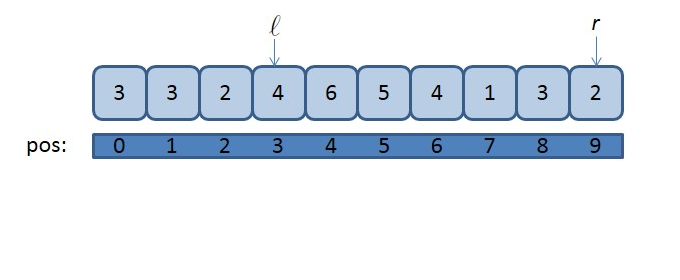
\includegraphics[width=8cm]{picture/sqrt_0.png}
\end{center}
\caption{$\sqrt{n}$ Buckets}
\label{sqrt_0}
\end{figure}

Dies bringt den Vorteil, das bei einem gegebenen Intervall nicht mehr das komplette Array durchsucht werden muss, sondern nur noch die entsprechenden Buckets. Hierbei m�ssen zwei F�lle unterschieden werden. \\
Fall 1: unser Intervall $(\ell, r)$ liegt genau am Anfang bzw. Ende der Buckets (Abb. \ref{sqrt_1}). In diesem Fall k�nnen wir einfach die entsprechenden Buckets durchsuchen um unser Minimum zu finden.

\begin{figure}[h]
\begin{center}
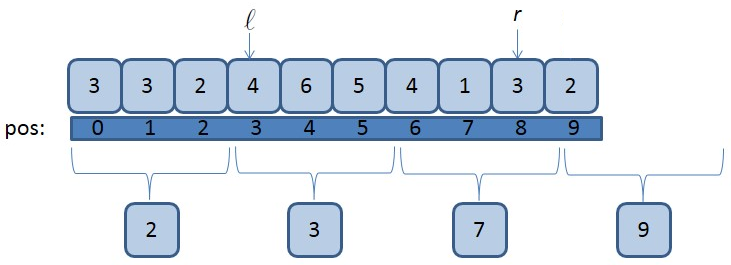
\includegraphics[width=8cm]{picture/sqrt_1.png}
\end{center}
\caption{Intervall genau in Buckets}
\label{sqrt_1}
\end{figure}

Bei Fall 2 hingegen, liegt unser Intervall nicht am Anfang bzw. Ende der Buckets was dazu f�hrt, das wir den Anfangs- bzw End-Bucket nicht benutzen d�rfen, da dort unter Umst�nden eine falsche Postion gespeichert ist und dies zu einem falschen Ergebnis f�hren w�rde (Abb. \ref{sqrt_2}).

\begin{figure}[h]
\begin{center}
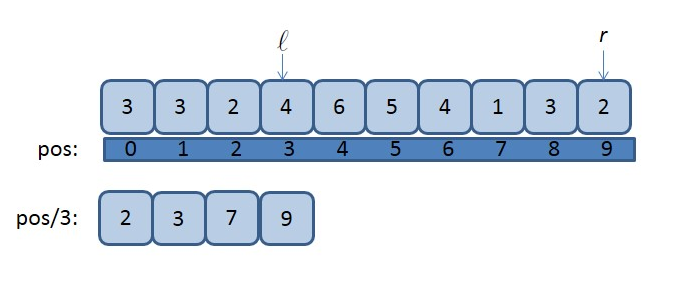
\includegraphics[width=8cm]{picture/sqrt_2.png}
\end{center}
\caption{Intervall in der Mitte der Buckets}
\label{sqrt_2}
\end{figure}

In diesem Fall m�ssen wir die Teile des Arrays, in denen wir keinen "`ganzen"' Bucket getroffen haben, noch einmal durchsuchen. \\
Kommen wir nun zur Laufzeitanalyse. Um unsere Bucketes zu initialisieren ben�tigen wir $\Oh(n)$, da dies in einem Durchlauf des Arrays geschehen kann. F�r eine Abfrage hingegen ben�tigen wir bei Fall 1 nur $\sqrt{n}$ Vergleiche. F�r Fall 2 hingegen kommen wir im worst case auf $[\sqrt{n} - 2]$ \footnote{\label{sqrt:1} f�r die Buckets die wir auf jeden Fall benutzen k�nnen} $+$ $[2\cdot(\sqrt{n}-1)]$ \footnote{\label{sqrt:2} f�r die Teile des Arrays die neu durchsucht werden m�ssen} was aus multipliziert zu $3 \cdot \sqrt{n} -4 $ wird. Dies liegt offensichtlich in $\Oh (\sqrt{n})$. 

Somit haben wir eine Preprocessingtime von $\Oh(n)$ und eine Querytime von $\Oh (\sqrt{n})$.

\subsection{Sparse Table}\label{spa}
Als n�chstes er�rtern wir den Sparse Table Algorithmus (STA). Der STA besteht im Wesentlichen aus zwei Phasen. In Phase 1 wird zun�chst eine Matrix $A$ mit $n$ Zeilen und $\lfloor \log n \rfloor +1$ Spalten erstellt.

Der ein oder andere Leser wird sich jetzt fragen, wieso brauchen wir nur $\lfloor \log n \rfloor +1$ Spalten? Dies l�sst sich am besten anhand eines Beispiels zeigen. Angenommen wir haben das Eingabearray aus Abb. \ref{sparse_0}.

\begin{figure}[h]
\begin{center}
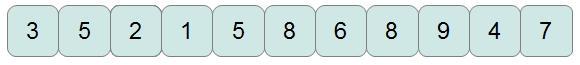
\includegraphics[width=6cm]{picture/sparse_0.png}
\end{center}
\caption{Eingabearray}
\label{sparse_0}
\end{figure}

Zun�chst ben�tigen wir die Zweierpotenz, welche mindestens die H�lfte des Arrays �berdeckt. In unserem Beispiel ist es die 8. Jetzt kommen wir zu dem Trick, und zwar benutzen wir nun die Tatsache das wenn wir zweimal diese Zweierpotenz benutzen, wir das Array komplett �berdecken k�nnen (Abb. \ref{sparse_01}).

\begin{figure}[h]
\begin{center}
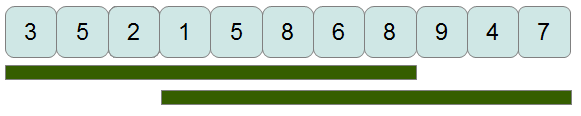
\includegraphics[width=6cm]{picture/sparse_01.png}
\end{center}
\caption{�berdeckung}
\label{sparse_01}
\end{figure}

Dadurch k�nnen wir das Minimum des Arrays ermitteln, indem wir jeweils das Minimum der beiden Zweierpotenzen bestimmen und davon einfach den kleineren Wert benutzen.
Diesen Trick benutzen wir nun um unsere Matrix $A$ aufzubauen. Im Wesentlichen baut sich $A$ folgenderma�en auf. Jede Zeile steht f�r die entsprechende Position im Array und die Spalten entsprechen einer Zweierpotenz (Abb. \ref{sparse_02} und \ref{sparse_03}).

\begin{figure}[h]
\begin{center}
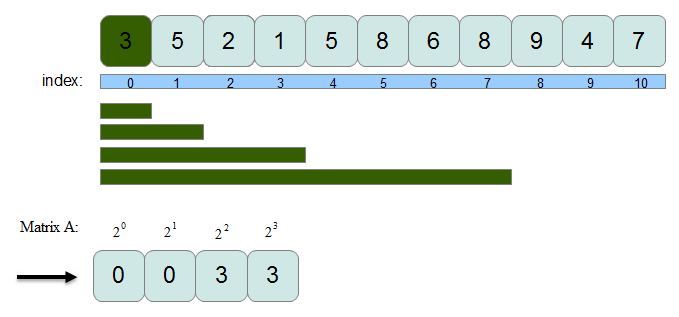
\includegraphics[width=10cm]{picture/sparse_02.png}
\end{center}
\caption{Erste Zeile Matrix $A$}
\label{sparse_02}
\end{figure}

\begin{figure}[h]
\begin{center}
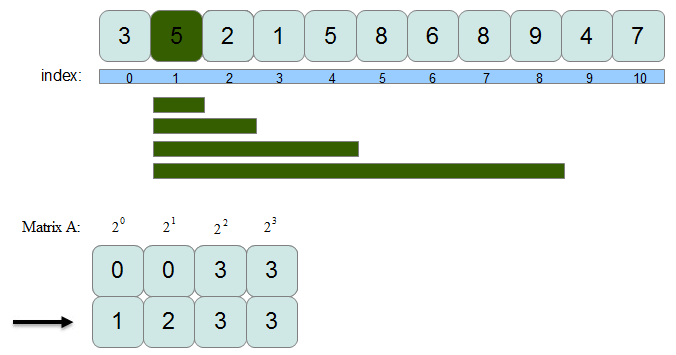
\includegraphics[width=10cm]{picture/sparse_03.png}
\end{center}
\caption{Zweite Zeile Matrix $A$}
\label{sparse_03}
\end{figure}

\newpage
Dies f�hren wir f�r jede Position im Array durch. Nun haben wir unsere "`Sparse Table"'\footnote{\label{sparse:1} sparse, da unsere Matrix $A$ nur $\lfloor \log n \rfloor +1$ Spalten besitzt, und nicht $n$ Spalten} erstellt und haben damit Phase 1 abgeschlossen.

Anzumerken ist noch das die Initialisierung der Matrix $A$ durch dynamische Programmierung optimiert werden kann. Dazu wird beim Berechnen der Zeilen nicht f�r jede Spalte das Array komplett durchlaufen, sondern nur noch der Teil des Array der noch nicht besucht wurde.

Kommen wir nun zur Phase 2. Hierbei benutzen wir nun das Intervall innerhalb unseres Arrays in welchem wir das Minimum suchen. Dazu gehen wir wie folgt vor: zun�chst suchen wir die Zweierpotenz, welche mindestens die H�lfte des Intervalls �berdeckt. Auch hier werden wir das Ganze durch ein einfaches Beispiel erl�utern.

Zun�chst sei unser Intervall zwischen Index 1 und 9 gegeben. Das hei�t unsere Zweierpotenz ist hier 8. Nun brauchen wir nur noch in den beiden entsprechenden Zeile unserer Matrix $A$ an Position 3\footnote{\label{sparse:2} da $2^3$ = 8} (Abb. \ref{sparse_04}) nachsehen und von den beiden Positionen das Minimum zu bestimmen.

\begin{figure}[h]
\begin{center}
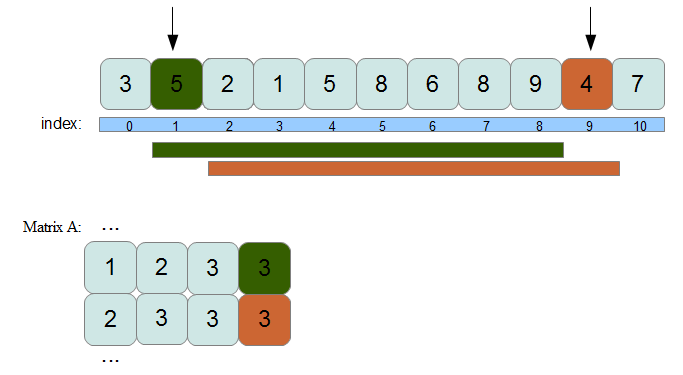
\includegraphics[width=10cm]{picture/sparse_04.png}
\end{center}
\caption{Abfrage}
\label{sparse_04}
\end{figure}

Zur Laufzeit k�nnen wir Folgendes festhalten: Offensichtlich ben�tigen wir f�r Phase 1 $\Oh(n \cdot \log n )$ um unsere Matrix $A$ zu berechnen. F�r eine Minimumbestimmung hingegen ben�tigen wir nur zwei Abfragen unserer Matrix $A$ was wir in $\Oh(1)$ schaffen. Daraus ergibt sich eine Laufzeit bei $m$ Abfragen von $\Oh (n \cdot \log n \cdot m)$.

\chapter{Skyline}

Als Anwendungsbeispiel haben wir das Skyline-Problem zur Bearbeitung erhalten. Es ist wie folgt beschrieben:

\section{Problemstellung}

Gegeben sei die zweidimensionale Projektion der Skyline einer Stadt aus verschieden hohen Geb�uden mit einheitlicher Breite. Uns als Werbeagentur wird es gestattet, auf eine zusammenh�ngende rechteckige Fl�che von Geb�uden der Skyline ein Werbebanner aufzukleben. Unsere Aufgabe ist es nun das Werbebanner m�glichst gro� zu w�hlen, sodass man es schon von Weitem sehen kann.

Beispielsweise sieht die Skyline der Stadt folgenderma�en aus:

\begin{figure}[h]
\begin{center}
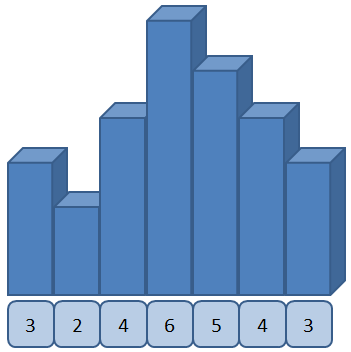
\includegraphics[width=5cm]{picture/skyline-test.png}
\end{center}
\caption{Skyline}
\label{skyline}
\end{figure}

\newpage
\section{Probleml�sung}

Wie schon in Abbildung \ref{skyline} zu sehen ist, l�sst sich eine gegebene Skyline einfach als Array von Geb�udeh�hen auffassen (im Beispiel 3,2,4,6,5,4,3). Doch wie kommt nun die Range Minimum Query ins Spiel? 

Unsere Idee ist die Folgende: Um die gr��tm�gliche Fl�che zu finden n�hern wir uns von unten nach oben der L�sung im divide \& conquer Prinzip an. Die erste M�glichkeit f�r ein Banner w�re �ber die gesamte Breite der zur Verf�gung stehenden Skyline ein Recheck anzusetzen.\\
Dieses Rechteck kann allerdings nur so hoch wie das niedrigste Geb�ude sein, da wir sonst ein freies Feld �ber diesem Geb�ude verdecken w�rden. Wir suchen also zun�chst das niedrigste Geb�ude in der Skyline, welches das Range Minimum unseres kompletten Eingabearrays darstellt.

\vspace{5mm}
\begin{figure}[h]
\begin{center}
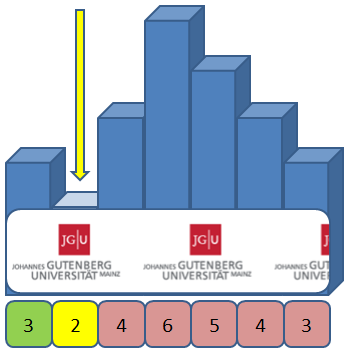
\includegraphics[width=5cm]{picture/skyline-left-right1.png}
\end{center}
\caption{Minimum suchen, Fl�che berechnen, Teilen}
\label{skylineteilen}
\end{figure}

Doch eventuell ist dieses Recheck nicht das gr��tm�gliche. Dann m�sste es ein gr��eres Rechteck links oder rechts von diesem Geb�ude geben. Auf jeden Fall geh�rt dann aber das kleinste Geb�ude nicht mehr dazu.\\
Wir suchen also ein gr��eres Rechteck in den verbleibenden Skylinefl�chen links (in Abbildung \ref{skylineteilen} gr�n dargestellt) und rechts (rot dargestellt) des bisherigen kleinsten Geb�udes, indem wir wieder das Range Mininum der linken Restskyline suchen, ein Rechteck mit dieser H�he und der restlichen Intervallbreite links konstruieren und dessen Fl�che mit der zuvor ermittelten maximalen Fl�che vergleichen.

Ebenso suchen wir in der rechten Restskyline das kleineste Geb�ude (Range Minimum) und bilden auch hier das Rechteck aus Restbreite rechts und H�he dieses Geb�udes.
Nun werden wieder diese beiden Range Minima Geb�ude weggelassen und in den verbleibenden restlichen vier Gebieten ebenso verfahren.

Nach diesem Schema verfahren wir solang bis die Teilprobleme nur noch eine Breite von eins haben und so keine weiteren Teilprobleme entstehen. Das bis dahin gefundene Rechteck mit maximaler Fl�che ist die L�sung des Problems.

\begin{figure}[h]
\begin{center}
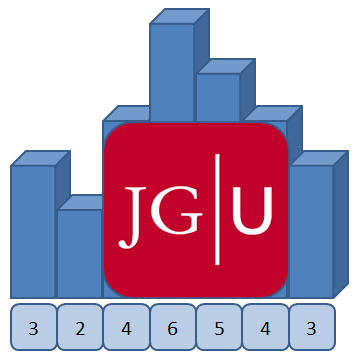
\includegraphics[width=5cm]{picture/skyline-end.png}
\end{center}
\caption{Gr��tm�gliche Fl�che = 16}
\label{skylineende}
\end{figure}



Unser Hauptalgorithmus besteht aus einer Queue von Teilproblemen und vier Schritten, die zyklisch auf den Teilproblemen der Queue ausgef�hrt werden, bis diese leer und das Ergebnis gefunden ist.

\vspace{3mm}
\begin{figure}[h]

\begin{tabular}[t]{lr}

\begin{minipage}{.6\textwidth}
\begin{verbatim}
while ( !Q.empty() ){
    //Intervall holen
    Interval(left, right) = Q.pop();
	
    //Minimum suchen
    min = RMQ( Interval(left, right) );
	
    //Fl�che vergleichen
    area = min * (right - left + 1);
    if ( area > max ) max = area;
	
    //Teilen rechts/links
    Q.add( Intervall(left, min - 1) );
    Q.add( Intervall(min + 1, right) );
}
\end{verbatim}
\end{minipage}

&

\begin{minipage}{.4\textwidth}
\begin{flushright}
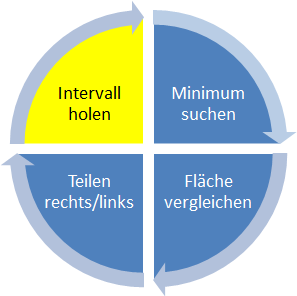
\includegraphics[width=40mm]{picture/algo-schritt4.png}
\end{flushright}
\end{minipage}
\\
\end{tabular}

\caption{Zyklischer Algorithmus}
\label{skylinealgo}
\end{figure}

\section{Optimierung}
\subsection{Teilprobleme ignorieren}
Wir k�nnen unseren L�sungsansatz noch optimieren. Dazu nutzen wir die Tatsache, dass wir eine maximale Geb�udeh�he gegeben hatten. Denn wenn wir die schon gefundene Maximalfl�che durch die Maximalh�he teilen (abgerundet), erhalten wir die L�nge von Teilproblemen, die wir ignorieren k�nnen. Da diese Teilprobleme nicht zu einer gr��eren Fl�che f�hren k�nnen.  Dazu sehen wir uns folgendes Beispiel an:

\begin{figure}[h]
\begin{center}
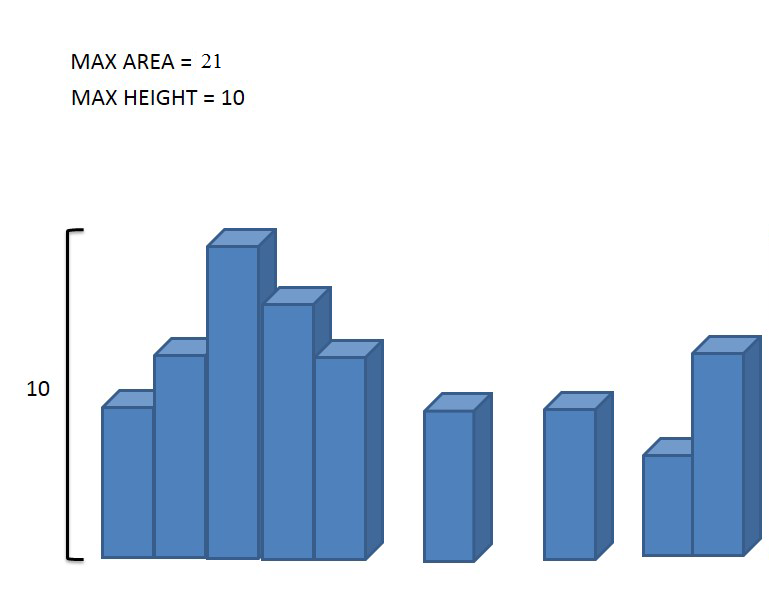
\includegraphics[width=6.5cm]{picture/optimierung_01.png}
\end{center}
\caption{Maximalh�he bei der Skyline}
\label{optimierung_01}
\end{figure}

Hier haben wir eine Maximalh�he von 10 und eine schon gefundene Fl�che von 21.
Daraus ergibt sich, dass wir Teilprobleme der L�nge 2 ignorieren k�nnen. In der folgenden Grafik haben wir Teilprobleme die ignoriert werden k�nnen in grau hinterlegt.
  
\begin{figure}[h]
\begin{center}
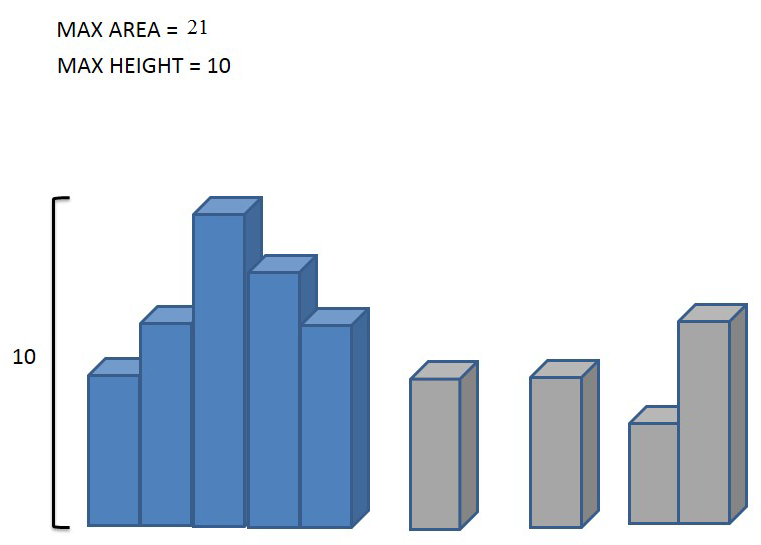
\includegraphics[width=6.5cm]{picture/optimierung_02.png}
\end{center}
\caption{Teilprobleme ignorieren}
\label{optimierung_02}
\end{figure}

Wie sich dies auf die Laufzeit auswirkt, ist schwer abzusch�tzen, da dies davon abh�ngt wie fr�h wir eine tempor�re maximale Fl�che finden.


\subsection{Parallelisierung}
Wie wir schon im Punkt \ref{spa} gezeigt haben, k�nnen wir eine Sparse Table in $\Oh( n \cdot \log n )$ berechnen. Nun stellt sich die Frage, geht dies nicht noch effizienter? \\
Ja, wenn wir Parallelisierung benutzen. Parallelit�t ist schon l�ngst Alltag geworden, seien es moderne Grafikkarten (Nvidia, AMD) oder Intels MIC\footnote{\label{optimierung:1}Many-Integrated-Core z.B. Xeon Phi Coprozessor}. 

Angenommen wir wollen nun unseren Sparse Table berechnen und haben mindestens so viele Threads wie Zeilen. Mit Hilfe einer geeigneten parallelen Sprache (CUDA, OpenCL oder Cilk Plus) k�nnen wir nun jede Zeile einem eigenen Thread zuweisen und verringern somit unsere Laufzeit drastisch (Abb. \ref{optimierung_03}). 
\begin{figure}[h]
\begin{center}
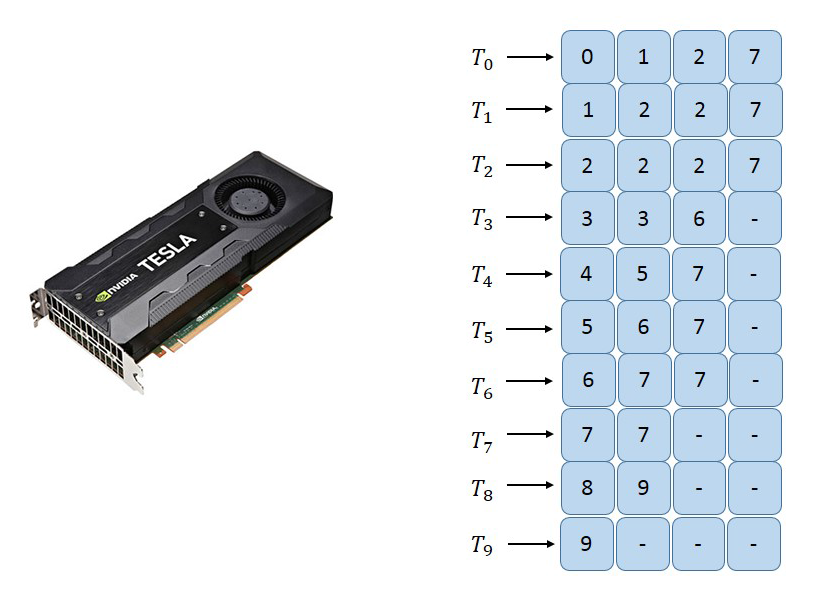
\includegraphics[width=10cm]{picture/optimierung_03.png}
\end{center}
\caption{Pro Zeile ein Thread}
\label{optimierung_03}
\end{figure}

Doch wir haben nicht immer mehr Threads als Zeilen. In diesem Fall werden die Zeilen zyklisch durchiteriert. Das hei�t jeder Thread berechnet mehrere Zeilen. Dies f�hrt zu einer allgemein optimierten Laufzeit von $\Oh (\frac{n}{T} \cdot \log n)$, wobei $T$ die Anzahl der Threads beschreibt.

\newpage
\section{Anhang: Sourcecode}

\begin{verbatim}

import java.io.BufferedReader;
import java.io.IOException;
import java.io.InputStreamReader;
import java.util.Arrays;
import java.util.LinkedList;
import java.util.Queue;

public class RMQ {

    /**
     * the main function.
     * @param args commandline args
     */
    public static void main(final String[] args) {

        BufferedReader reader = new BufferedReader(
                                new InputStreamReader(System.in));
        try {
            while (true) {
                String line = reader.readLine();

                if (line.startsWith("END")) {
                    break;
                }

                // first line n m
                String[] splittedLine = line.split(" ");
                long n = Long.parseLong(splittedLine[0]);
                int m = Integer.parseInt(splittedLine[1]);

                // second line h
                line = reader.readLine();
                String[] strh = line.split(" ");
                long[] h = new long[m];
                for (int i = 0; i < m; i++) {
                    h[i] = Long.parseLong(strh[i]);
                }

                // start with skyline
                long[] r = new long[(int) n];
                r = generateH(n, m, h);
                System.out.println(skyline(r, n));
            }

            reader.close();
        } catch (IOException e) {
            e.printStackTrace();
        }
    }

    /**
     * Solves the skyline problem. A skyline is the outline formed by a group of
     * buildings against the sky. A certain city has a beautiful skyline that's
     * visible to everybody as they approach it by car. You have bought the
     * rights to place an advertisement over it, and you would like to do so
     * while preserving the shape of the city. The skyline is formed by n
     * buildings, all with a width of 1 and each with a different height. You
     * will place your ad on a rectangle of maximum area that is fully contained
     * within the interior of the skyline.
     *
     * @param r   the array containing the building heights
     * @param n   the number of buildings
     * @return the maximum area on the buildings
     */
    public static long skyline(final long[] r, final long n) {
        if (n == 1) {
            return r[(int) n - 1];
        } else {
            int[][] sparseTable = process2(r, r.length);

            int minimum = min(0, (int) n - 1, r, sparseTable);
            Queue<int[]> interval = new LinkedList<int[]>();
            long area = n * r[minimum];

            if (minimum == 0) {
                if (r[0] > area) {
                    area = r[0];
                }
            } else {
                int[] links = new int[2];
                links[0] = 0;
                links[1] = minimum - 1;
                interval.add(links);
            }

            if (minimum == n - 1) {
                if (r[minimum] > area) {
                    area = r[minimum];
                }
            } else {
                int[] rechts = new int[2];
                rechts[0] = minimum + 1;
                rechts[1] = (int) n - 1;
                interval.add(rechts);
            }

            while (!interval.isEmpty()) {

                int[] tmp = interval.poll();
                int minTmp = min(tmp[0], tmp[1], r, sparseTable);

                long tmpArea = r[minTmp] * (tmp[1] - tmp[0] + 1);
                if (tmpArea > area) {
                    area = tmpArea;
                }

                // links
                if (tmp[0] == minTmp || tmp[0] == minTmp - 1) {
                    if (r[tmp[0]] > area) {
                        area = r[tmp[0]];
                    }
                } else {
                    int[] linksTmp = new int[2];
                    linksTmp[0] = tmp[0];
                    linksTmp[1] = minTmp - 1;
                    interval.add(linksTmp);
                }

                // rechts
                if (minTmp == tmp[1] || minTmp + 1 == tmp[1]) {
                    if (r[tmp[1]] > area) {
                        area = r[tmp[1]];
                    }
                } else {
                    int[] rechtsTmp = new int[2];
                    rechtsTmp[0] = minTmp + 1;
                    rechtsTmp[1] = tmp[1];
                    interval.add(rechtsTmp);
                }
            }
            return area;
        }
    }

    /**
     * used to preprocess the n heights out of the m given start vectors in h.
     *
     * @param n
     *            number of buildings
     * @param m
     *            number of elements in h
     * @param h
     *            start vector with m inital heights
     * @return the buildingheights array with length n
     */
    public static long[] generateH(final long n, final int m, final long[] h) {
        int j = 0;
        int s = 0;
        long[] r = new long[(int) n];
        for (int i = 0; i <= n - 1; ++i) {
            r[i] = h[j];
            s = (j + 1) % m;
            h[j] = ((h[j] ^ h[s]) + 13) % 835454957;
            j = s;
        }
        return r;
    }

    /**
     * RMQ function. searches the range minimum in r in O(1)
     *
     * @param i   start of the query range
     * @param j   end of the query range
     * @param r   the range to be searched in
     * @param M   the preprocessed sparse matrix
     * @return the index of the minimum in r between i and j
     */
    public static int min(final int i, 
                            final int j, 
                            final long[] r, 
                            final int[][] M) {

        int k = (int) ((Math.log(j - i + 1) / Math.log(2)));
        int mini = M[(int) (j - (1 << k) + 1)][k]; // 1<<k = 2^k

        if (r[(int) M[i][k]] <= r[(int) mini]) {
            return M[i][k];
        } else {
            return mini;
        }
    }

    /**
     * preprocesses the array A for quicker RMQ in O(n*log(n)).
     *
     * @param A  the given array
     * @param N  size of the array
     * @return   the sparse Matrix used in RMQ
     */
    public static int[][] process2(final long[] A, final int N) {
        int i, j;

        int[][] M = new int[N][(int) Math.ceil(Math.log(N) / Math.log(2)) + 1];
        // initialize M for the intervals with length 1
        for (i = 0; i < N; i++) {
            M[i][0] = i;
        }
        // compute values from smaller to bigger intervals
        for (j = 1; 1 << j <= N; j++) {
            for (i = 0; i + (1 << j) - 1 < N; i++) {
                if (A[(int) M[i][j-1]] < A[(int) M[i + (1 << (j - 1))][j-1]]){
                    M[i][j] = M[i][j - 1];
                } else {
                    M[i][j] = M[i + (1 << (j - 1))][j - 1];
                }
            }
        }
        return M;
    }

    /**
     * function to visualize the skyline.
     *
     * @param r  the array with the building heights
     */
    public static void print(final long[] r) {
        // find max in array
        long n = r.length;
        long[] neu = new long[(int) n];
        neu = r.clone();
        Arrays.sort(neu);
        long maxheight = neu[(int) (n - 1)];

        // draw skyline
        for (long i = maxheight; i >= 1; i--) {
            System.out.print("|");
            for (long k = 0; k < n; k++) {
                if (r[(int) k] / i > 0) {
                    System.out.print("�??|");
                } else {
                    System.out.print(" |");
                }
            }
            System.out.println();
        }
        System.out.print("|");
        for (int i = 0; i < n; i++) {
            System.out.print(i / 10 + "|");
        }
        System.out.println();
        System.out.print("|");
        for (int i = 0; i < n; i++) {
            System.out.print(i % 10 + "|");
        }
        System.out.println();
    }
}


\end{verbatim}


%% Literaturverzeichnis
\addcontentsline{toc}{chapter}{Literaturverzeichnis}
\bibliography{sample}

\end{document}
